\section{Results} \label{sec:results}

The SM hypothesis tested in this analysis is the existence of the SM non-resonant di-Higgs process, probed via the WW$\gamma\gamma$ phase space. Additionally, BSM hypotheses are tested in the context of the 
EFT framework described in Section \ref{sec:EFT_Description}, including a di-Higgs process whose production cross section is altered due to the modification 
of the di-Higgs self-coupling, coupling of two Higgs bosons to two top quarks, and a group of 20 EFT benchmark nodes corresponding to modifications 
of $\kappa_{\lambda}$, $\kappa_{t}$, $c_{2}$, $c_{g}$, $c_{2g}$ defined in Tab. \ref{tab:eft_bench}. 

Expected (observed) results are obtained by performing a simultaneous likelihood fit of the signal and 
background templates to Asimov (observed) data, in categories defined by selections from a multiclassifier DNN in the SL final state, a combination 
of two binary DNN's in the FH final state, and a group of cut based selections in the FL final state. For the $\kappa_{\lambda}$ scan, the same categorization methods are used as for the 
SM case, but applied to three HH simulated samples corresponding to $\kappa_{\lambda}$ = [1, 2.45, 5], where a weighted linear combination and shape interpolation of the three is made in order to estimate 
the expected yield and shape for $\kappa_{\lambda}$ hypotheses between -30 and 30. The effects of anomalous $\kappa_{\lambda}$ values on the Higgs boson branching ratios and on the single Higgs cross sections are taken into account using the modeling provided in Ref.~\cite{Degrassi:2016wml} and \cite{Maltoni:2017ims}.

For the $c_{2}$ scan, a similar approach is taken but with the use of 6 EFT signal models obtained via a reweighting of 4 NLO samples. 
The 20 EFT benchmark node results are extracted in categories defined based on a parametric DNN in the SL final state, and a reweighting of SM MC events for the FH and FL final states.  

As it is not possible to observe evidence of an SM HH signal given the sensitivity of the analysis on the available dataset, a modified frequentist method $CL_s$ \cite{CLS1, CLS2} is used to 
calculate 95\% confidence-level ($CL_{s}$) exclusion limits with the asymptotic approximation \cite{Cowan:2010js}. This method is applied in order to determine the upper limit 
on the production cross section of each signal hypothesis. Each upper limit is extracted by positively scaling the corresponding 
HH signal model until it is incompatibile with the background-only hypothesis (expected), or data (observed), at a 95\% $CL_{s}$.   

Combining the SL results with the FL and FH WW$\gamma\gamma$ (+ZZ$\gamma\gamma$+bb$\gamma \gamma$ for fully hadronic case) channels leads to the combined
Run 2 results shown in Table \ref{tab:Run2Results}.

\begin{table}[h!]
  \begin{center}
    \begin{tabular}{c|c|ccccc}
      \hline
        & Observed limit & $-2\sigma$ & $-1\sigma$ & Expected Limit & $+1\sigma$ & $+2\sigma$ \\ \hline
          Fully-Leptonic &  280   &   81 & 120 & 190 & 330 & 550  \\ \hline
          Fully-Hadronic &  310  &   70 & 98 & 140 & 230 & 350   \\ \hline
          Semi-Leptonic  &  71  &   30 & 42 & 64 & 110 & 170 \\ \hline
          Combination    &  97  &   25 & 35 & 53 & 86 & 130  \\ \hline
          \end{tabular}
  \end{center}
  \caption{Full Run2 Combination results, including SL, FL and FH categories,
  on $\frac{\sigma(HH)}{\sigma_{SM}(HH)}$, assuming an NLO standard model cross section of about 31.05 fb. Results have been rounded to two significant figures.}
  \label{tab:Run2Results}
\end{table}  

A combined median value of 97 (53 expected) times the NLO approximation of the standard model gluon gluon HH cross section is obtained, considering a standard model cross section of 31.05 fb. 

The combined $\kappa_{\lambda}$ scan is shown in Figure \ref{fig:Combined_kl}, with each category and the combined median limit values shown
in Figure \ref{fig:Channel_kl}. Note that the theory prediction line, drawn in red, represents the predicted HH cross section value for a certain value of $\kappa_{\lambda}$.

As shown in Figure \ref{fig:Combined_kl}, an observed (expected) constraint on the Higgs self-coupling of about -26 (-14) to 24 (18) times its standard model value 
is obtained at a 95\% CL. 

The combined $c_{2}$ scan is shown in Figure \ref{fig:Combined_c2}, with each category and the combined median limit values shown
in Figure \ref{fig:Channel_c2}. Note that the theory prediction line, drawn in red, represents the predicted HH cross section value for a certain value of $c_{2}$.

As shown in Figure \ref{fig:Combined_c2}, an observed (expected) constraint on the coupling constant magnitude of two top quarks to two Higgs bosons of about
-2.4 (-1.8) to 2.9 (2.2) is extracted at a 95\% CL.

Finally, the observed (expected) upper limits on the production cross section of the 20 EFT benchmark scenarios defined in Tab. \ref{tab:eft_bench} are shown separately for each WW$\gamma\gamma$ final state in Figure \ref{fig:20_EFT_benchmark_results_perchannel}, and in the combined case in 
Fig.\ref{fig:20_EFT_benchmark_results_all}, where the combined results range from 1.7 - 6.2 (1.0 - 3.9) pb. 

\begin{figure}[!htbp]
  \centering
  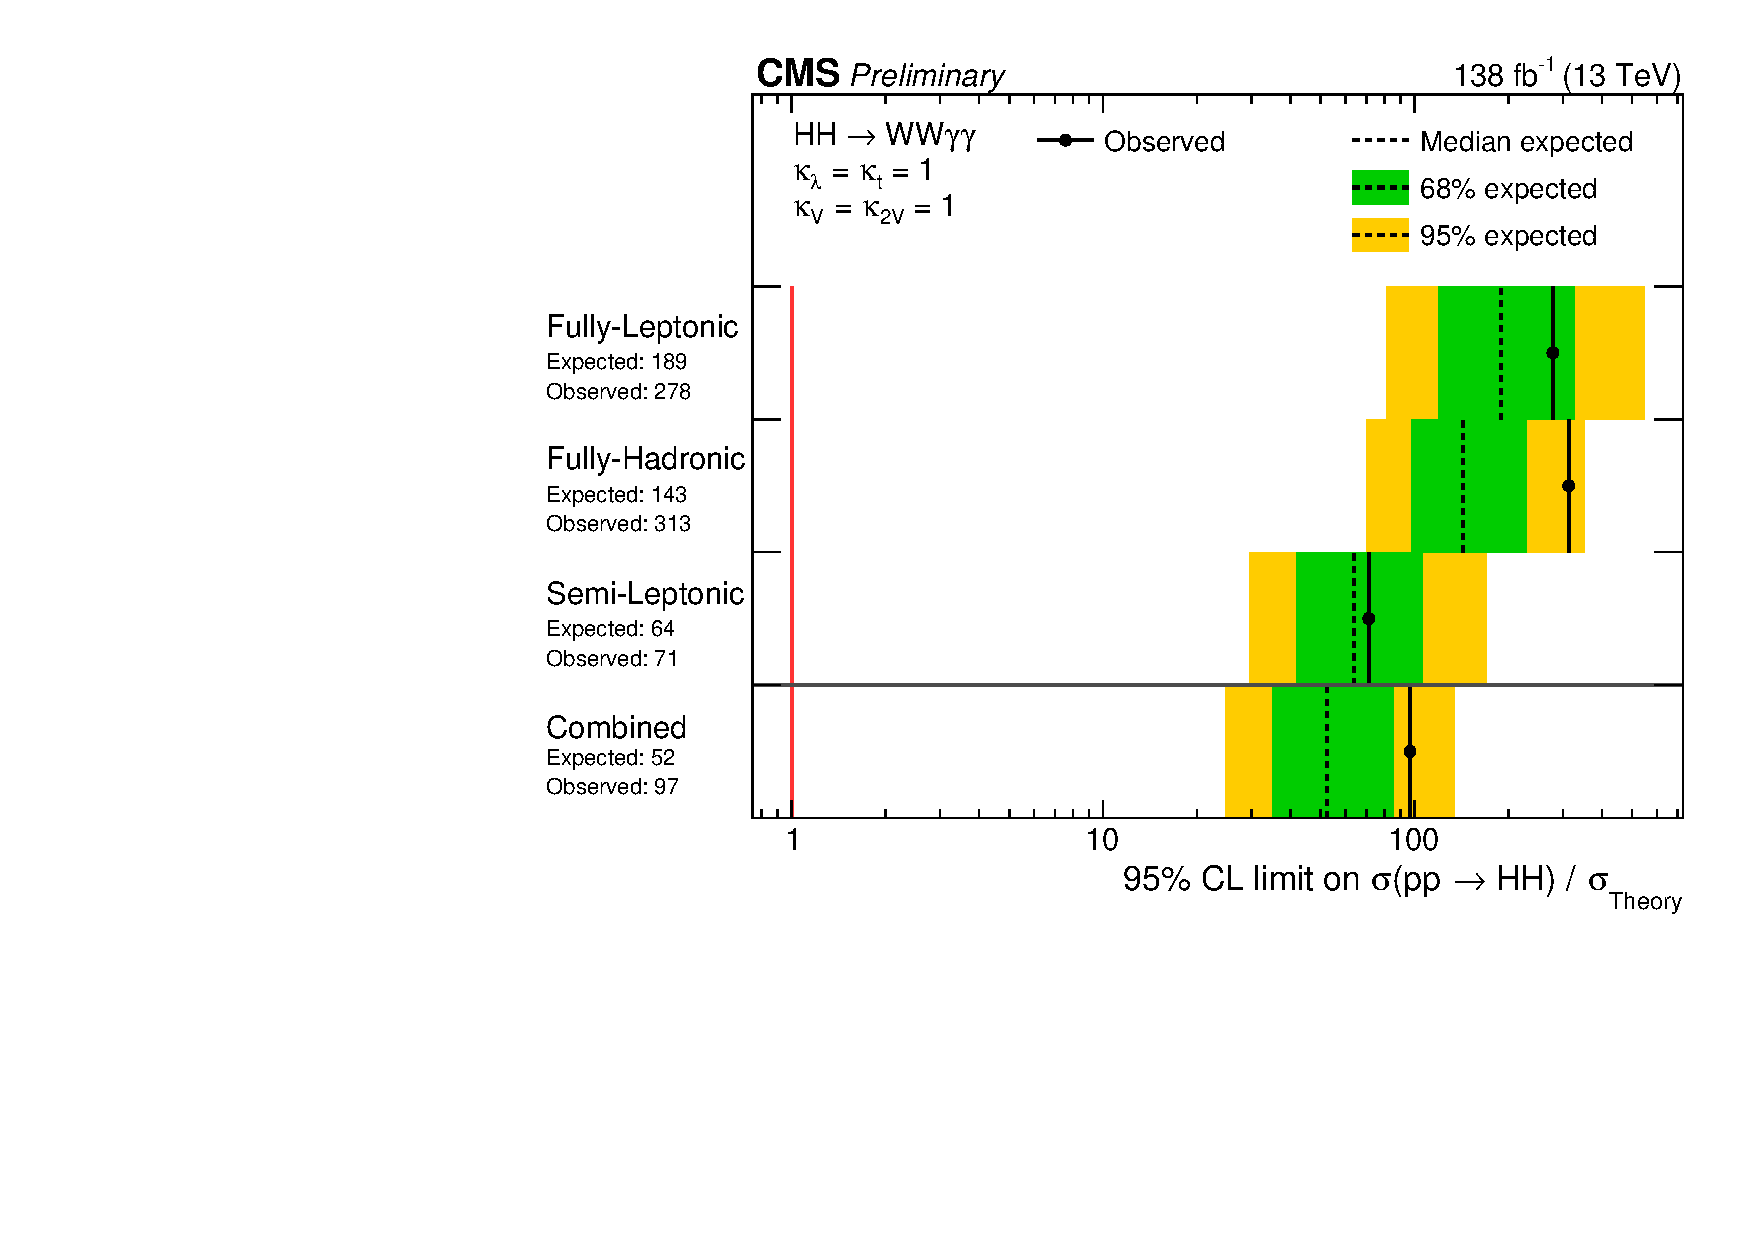
\includegraphics[width=0.9\textwidth]{Sections/HHWWgg/images/Results/All_limits.pdf}
  \caption{Run 2 95\% $CL_{s}$ limits on HH gluon gluon fusion production with respect to $\sigma_{SM}^{NLO} \approx $ 31.05fb. Note that the red line at one corresponds to the SM prediciton.}
  \label{fig:Run2SMNLOCombined}
\end{figure}

\begin{figure}[!htbp]
  \setcounter{subfigure}{0}
  \centering
  \subfloat[Per channel]{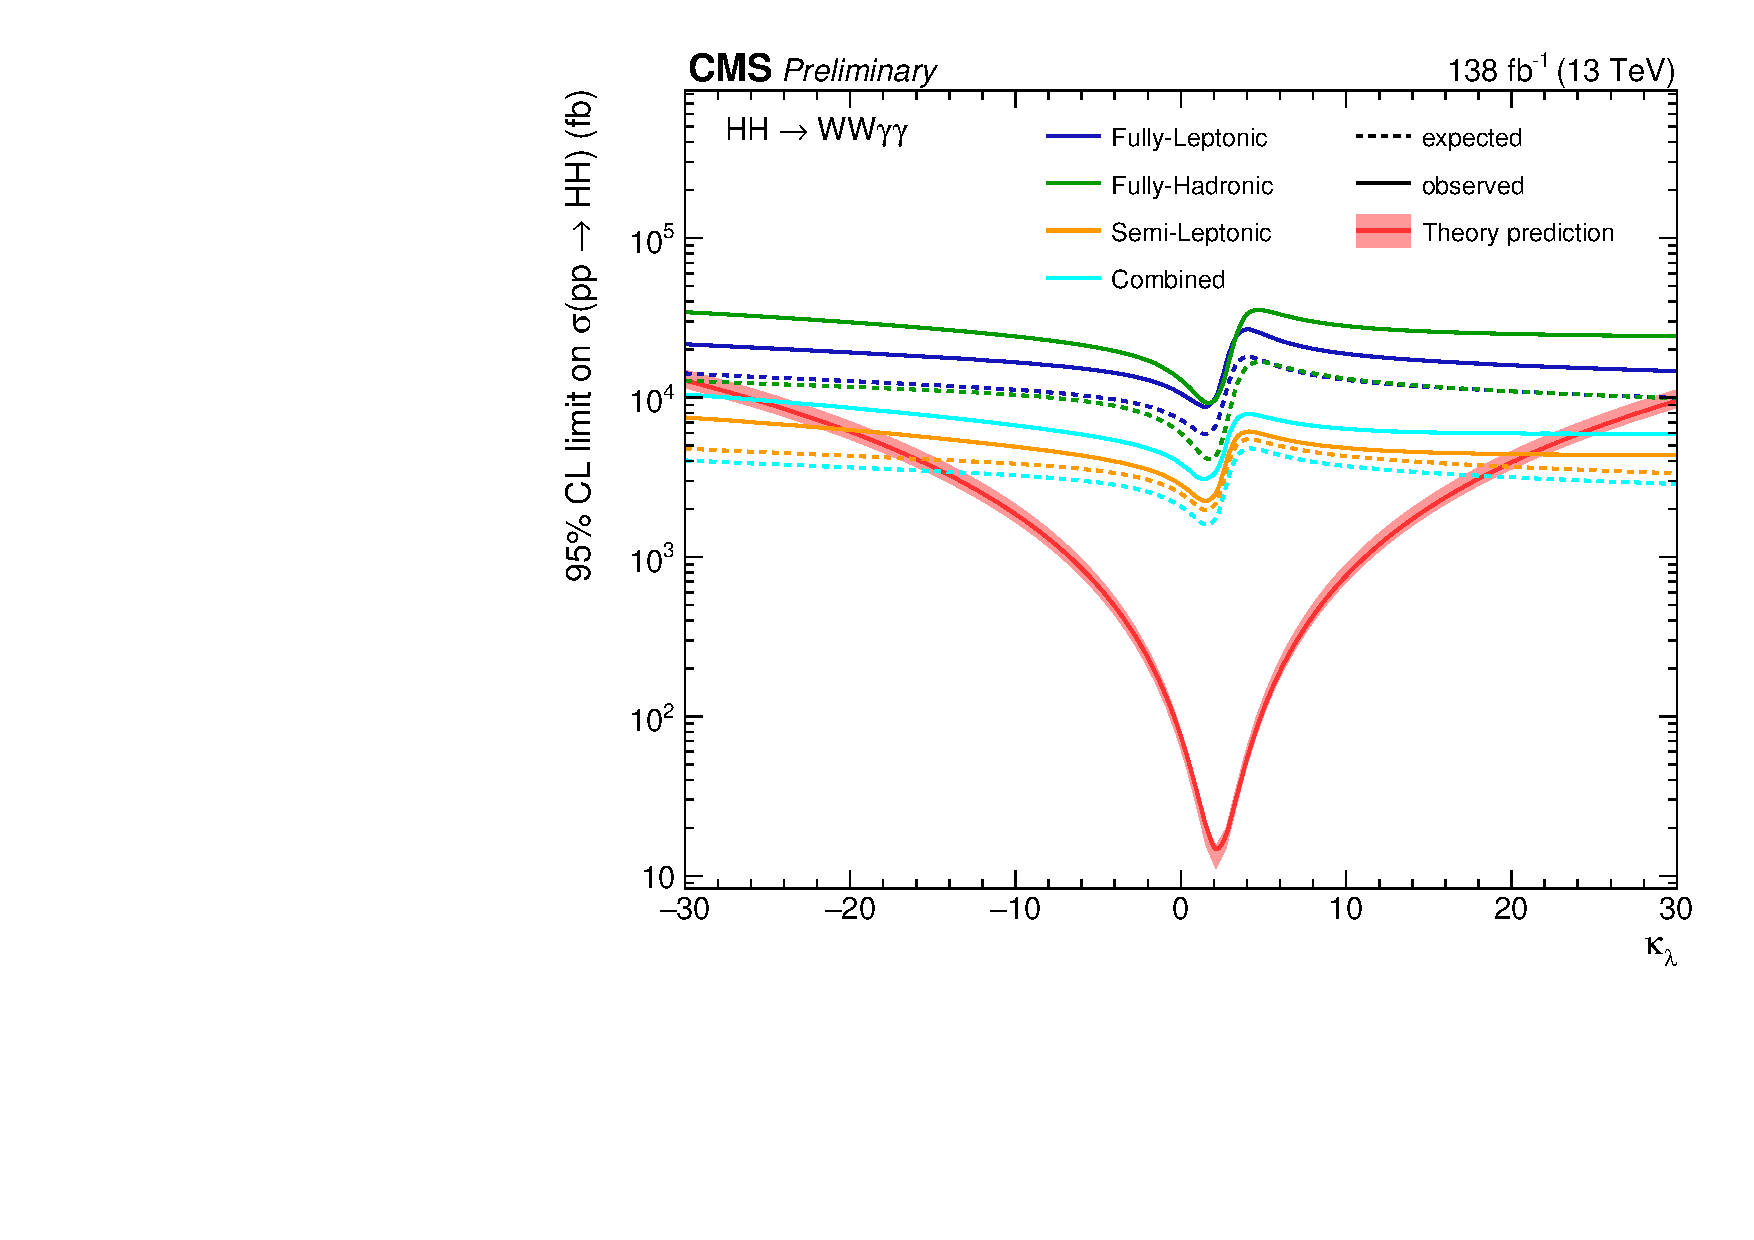
\includegraphics[width=0.45\textwidth]{Sections/HHWWgg/images/Results/kl_Comparison.pdf} \label{fig:Channel_kl}} 
  \qquad
  \subfloat[Combined]{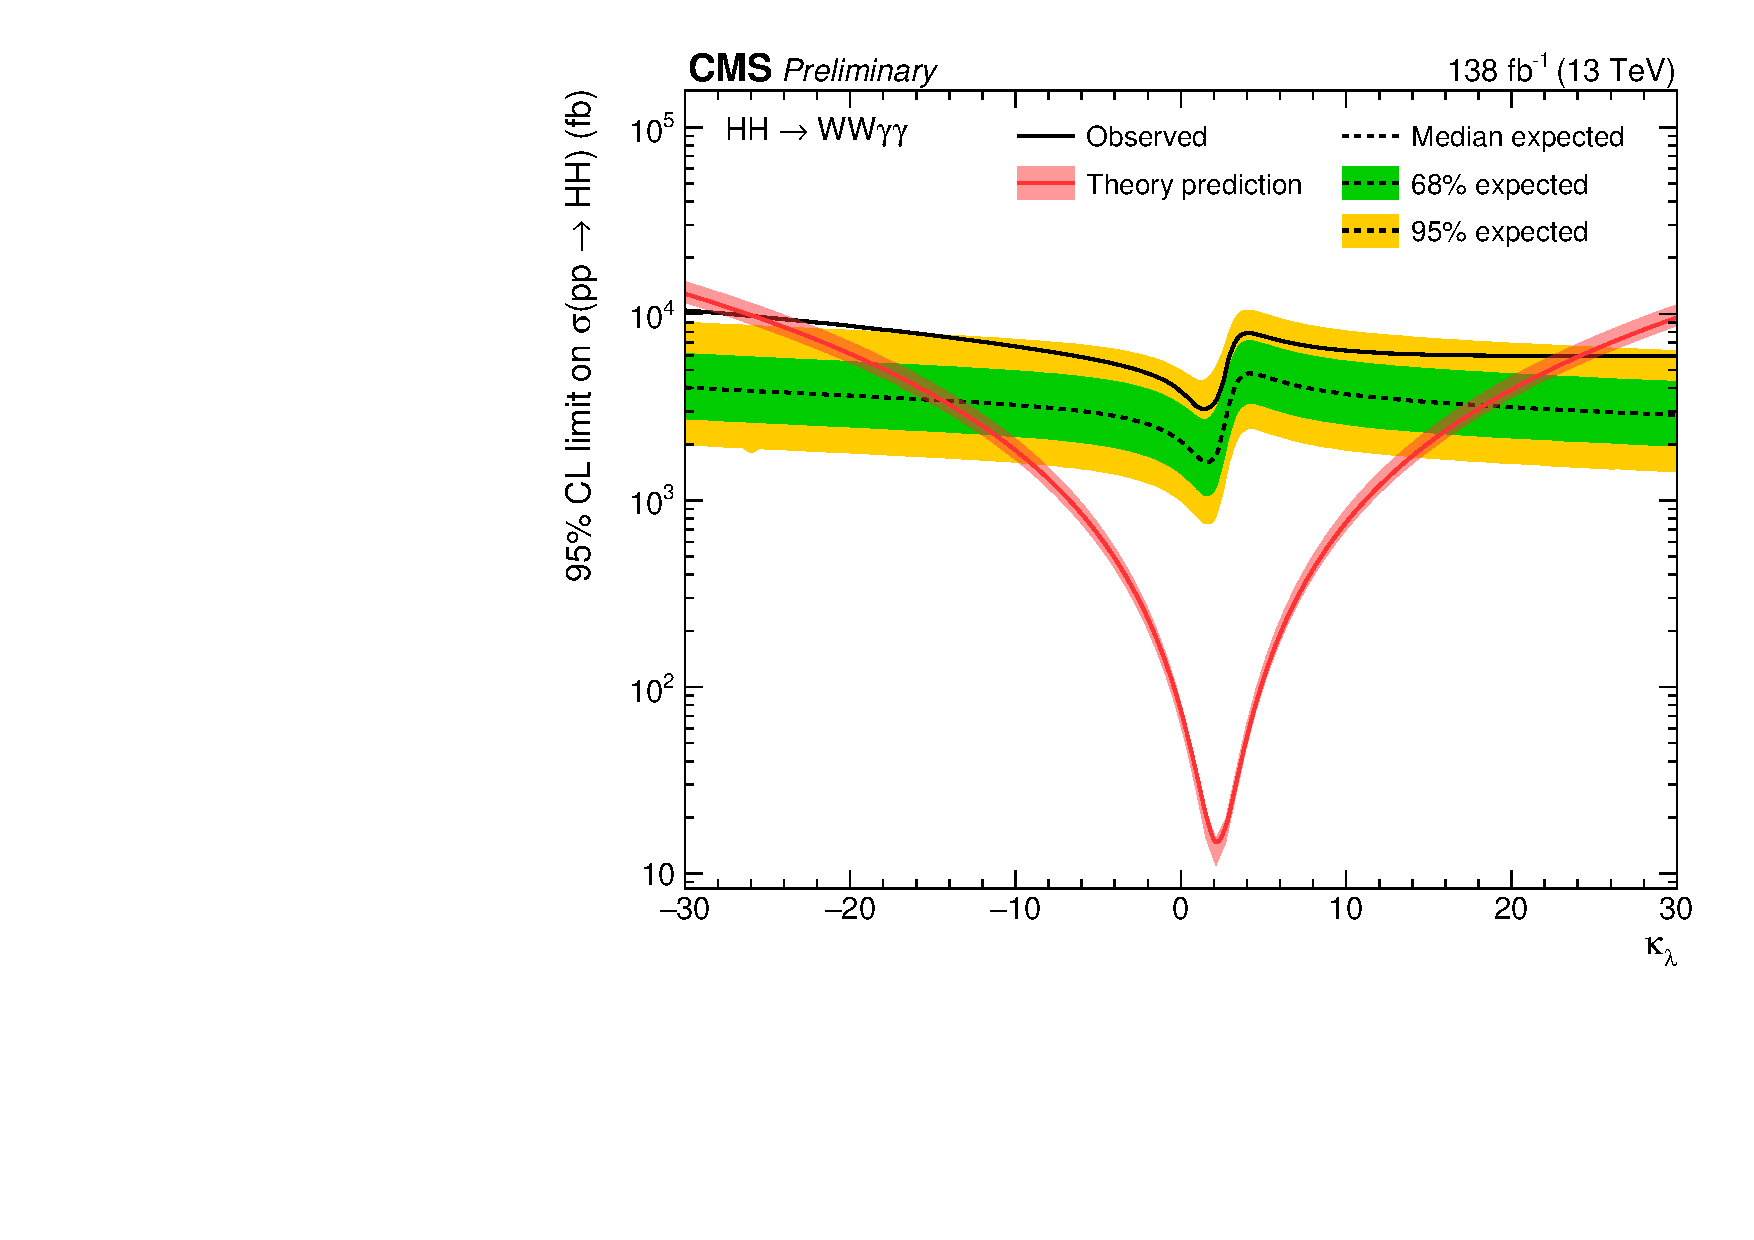
\includegraphics[width=0.45\textwidth]{Sections/HHWWgg/images/Results/HHWWgg_kl_Scan.pdf}\label{fig:Combined_kl}}
  \caption{95\% $CL_{s}$ upper limit scan of $\kappa_{\lambda}$ hypotheses from -30 to 30. Note that the red curves correspond to theoretical cross section predictions for each given $\kappa_{\lambda}$ hypothesis.}
  \label{fig:kl_scan}
\end{figure}

\begin{figure}[!htbp]
  \setcounter{subfigure}{0}
  \centering
  \subfloat[Per channel]{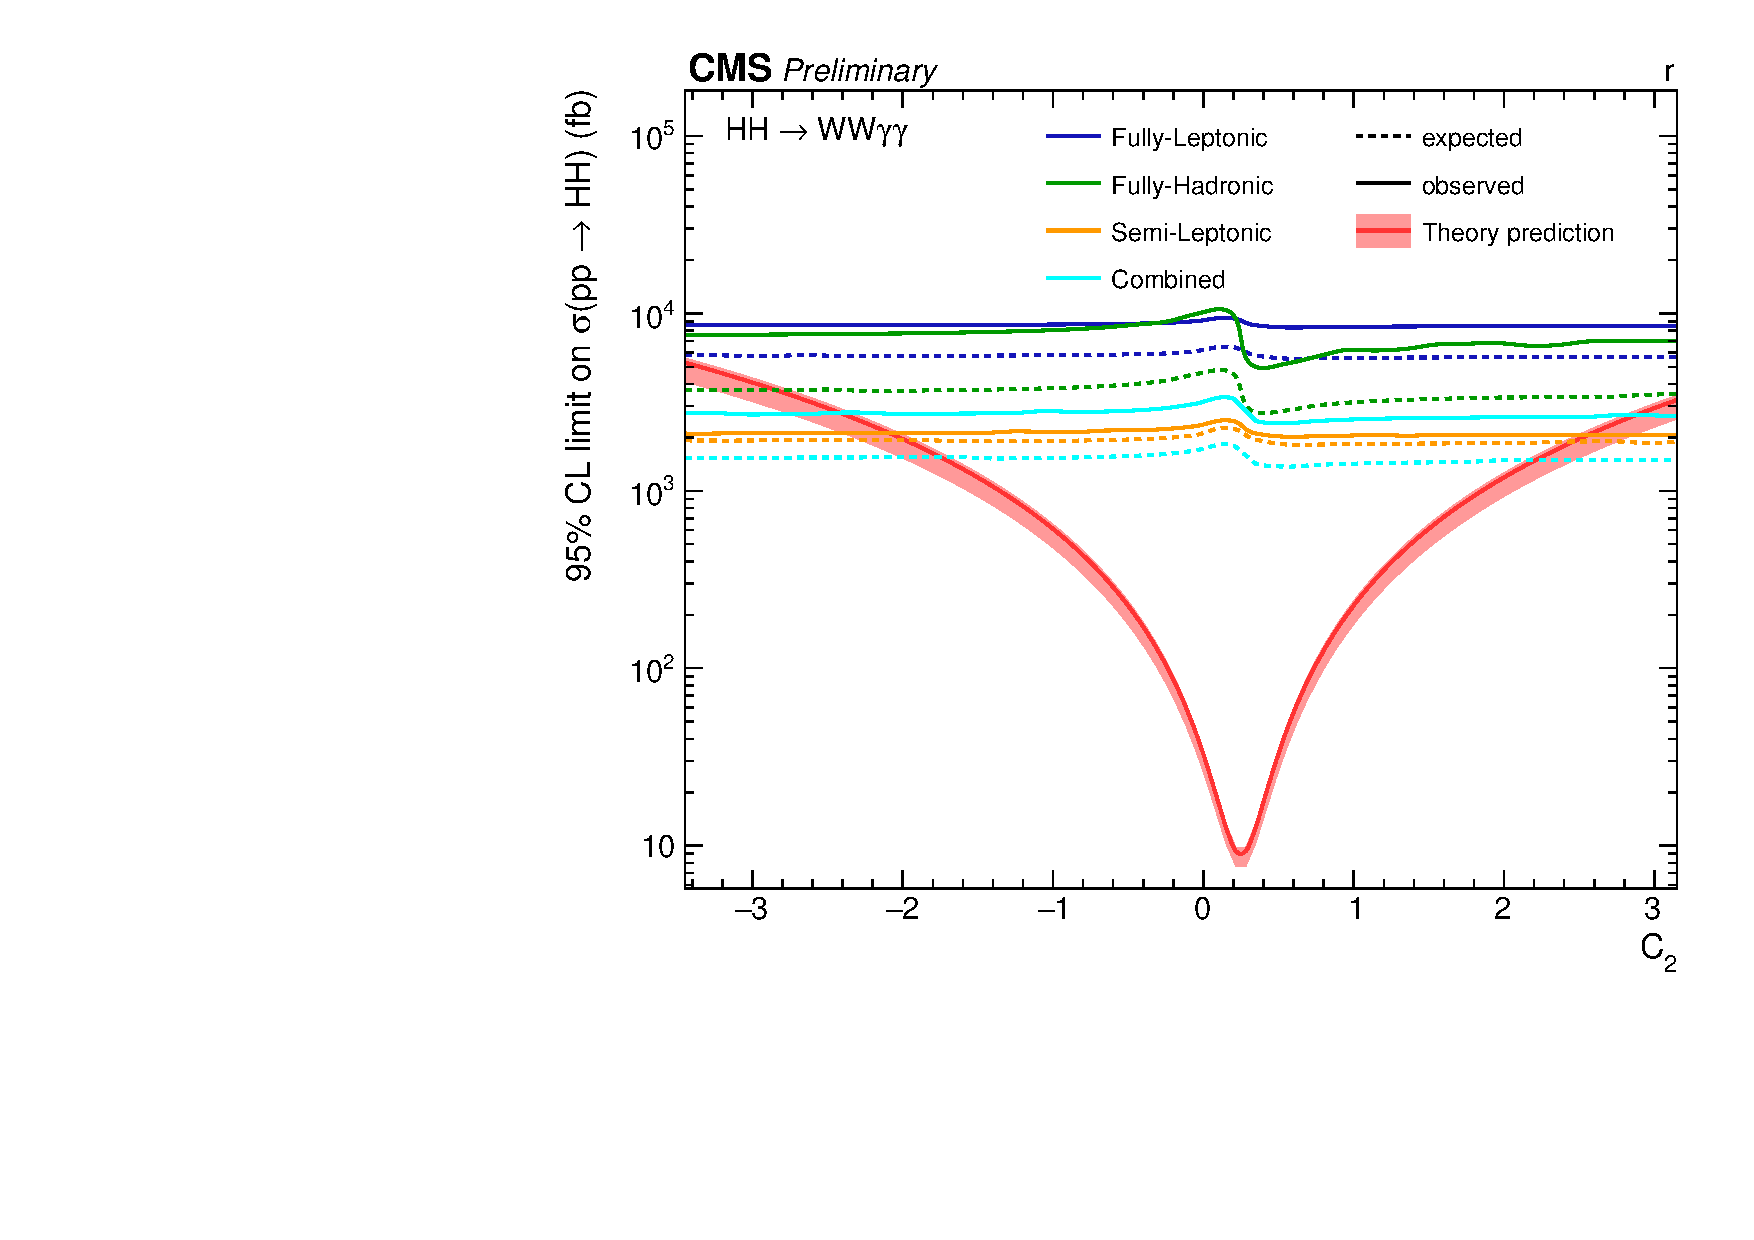
\includegraphics[width=0.45\textwidth]{Sections/HHWWgg/images/Results/C2_Comparison.pdf}\label{fig:Channel_c2}} 
  \qquad
  \subfloat[Combined]{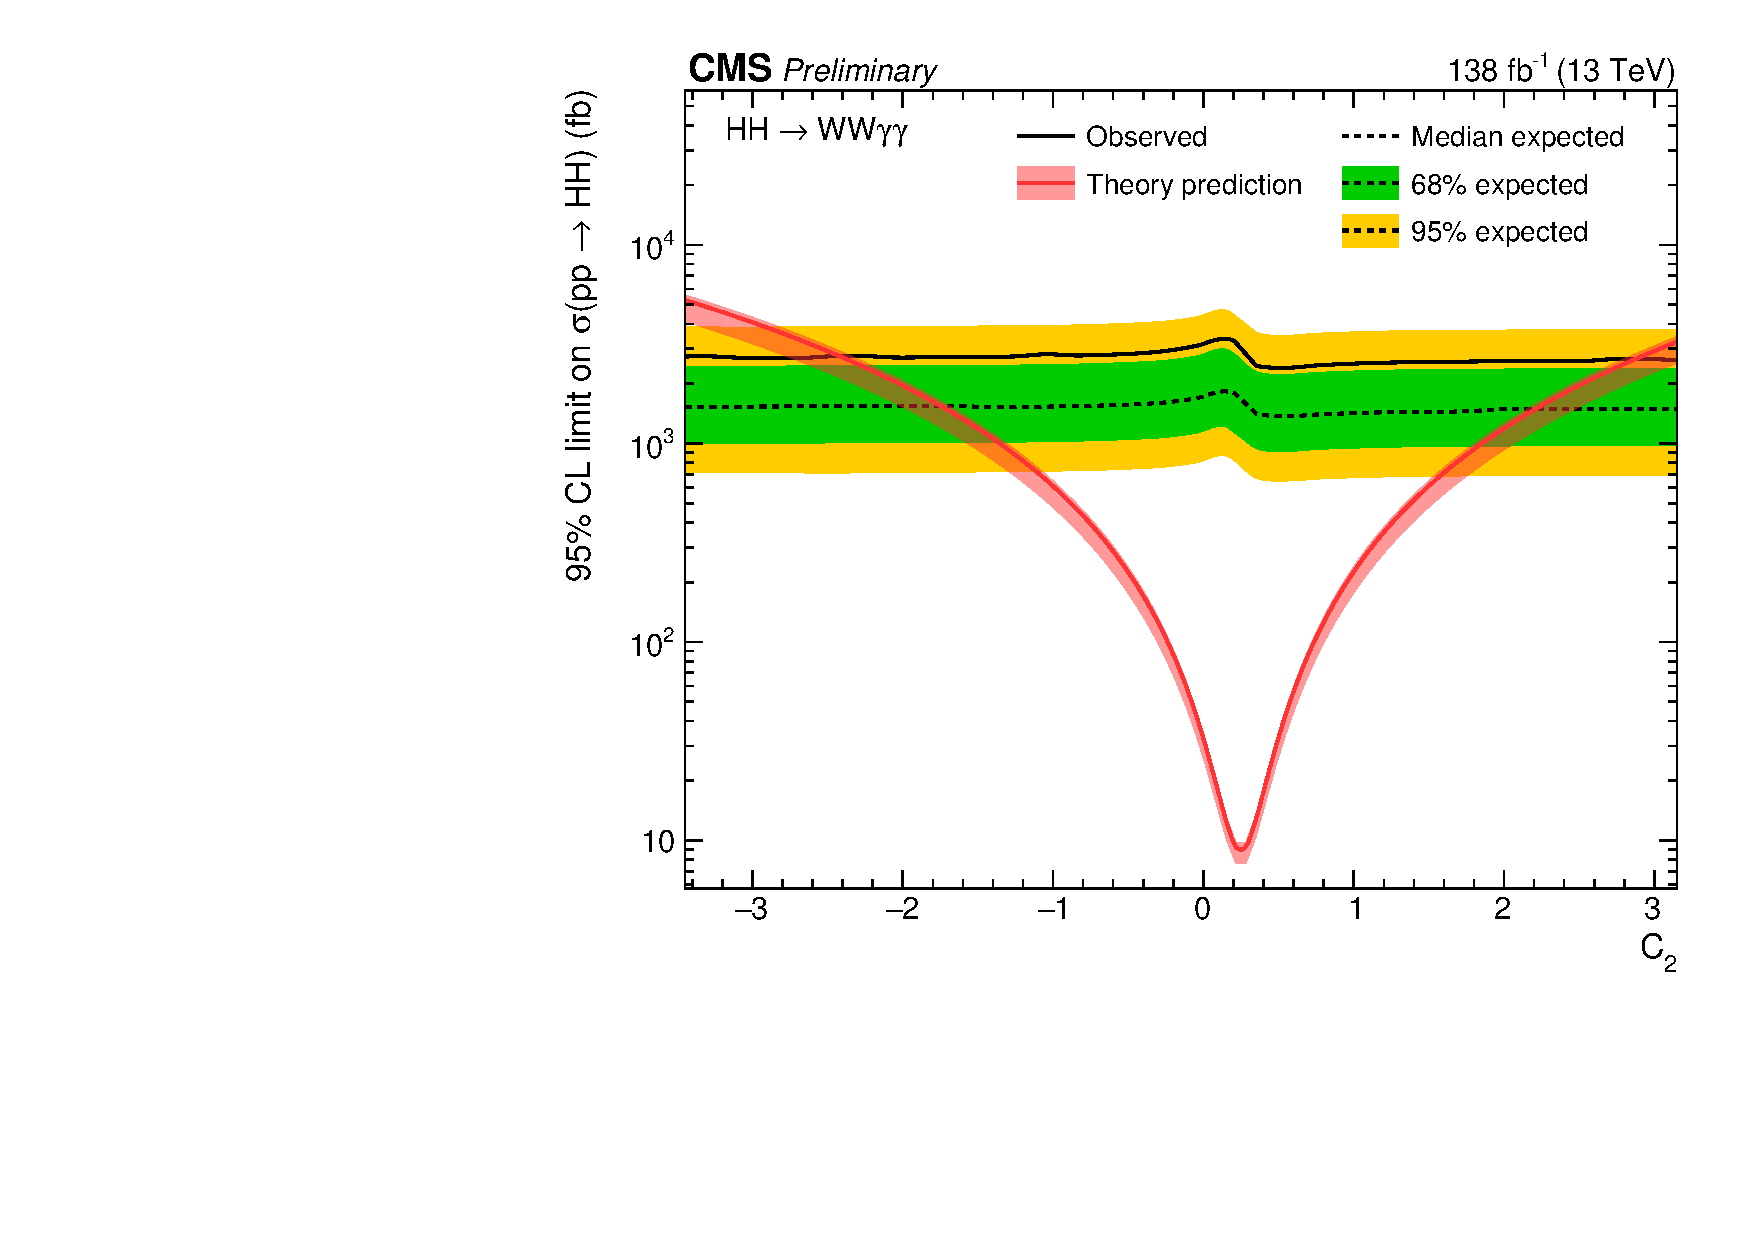
\includegraphics[width=0.45\textwidth]{Sections/HHWWgg/images/Results/HHWWgg_C2_Scan.pdf}\label{fig:Combined_c2}}
  \caption{95\% $CL_{s}$ upper limit scan of $c_{2}$ hypotheses from -3 to 3. Note that the red curves correspond to theoretical cross section predictions for each given $c_{2}$ hypothesis.}
  \label{fig:c2_scan}
\end{figure}

\begin{figure}[!htbp]
    \setcounter{subfigure}{0}
    \centering
    \subfloat[Semi-Leptonic channel]{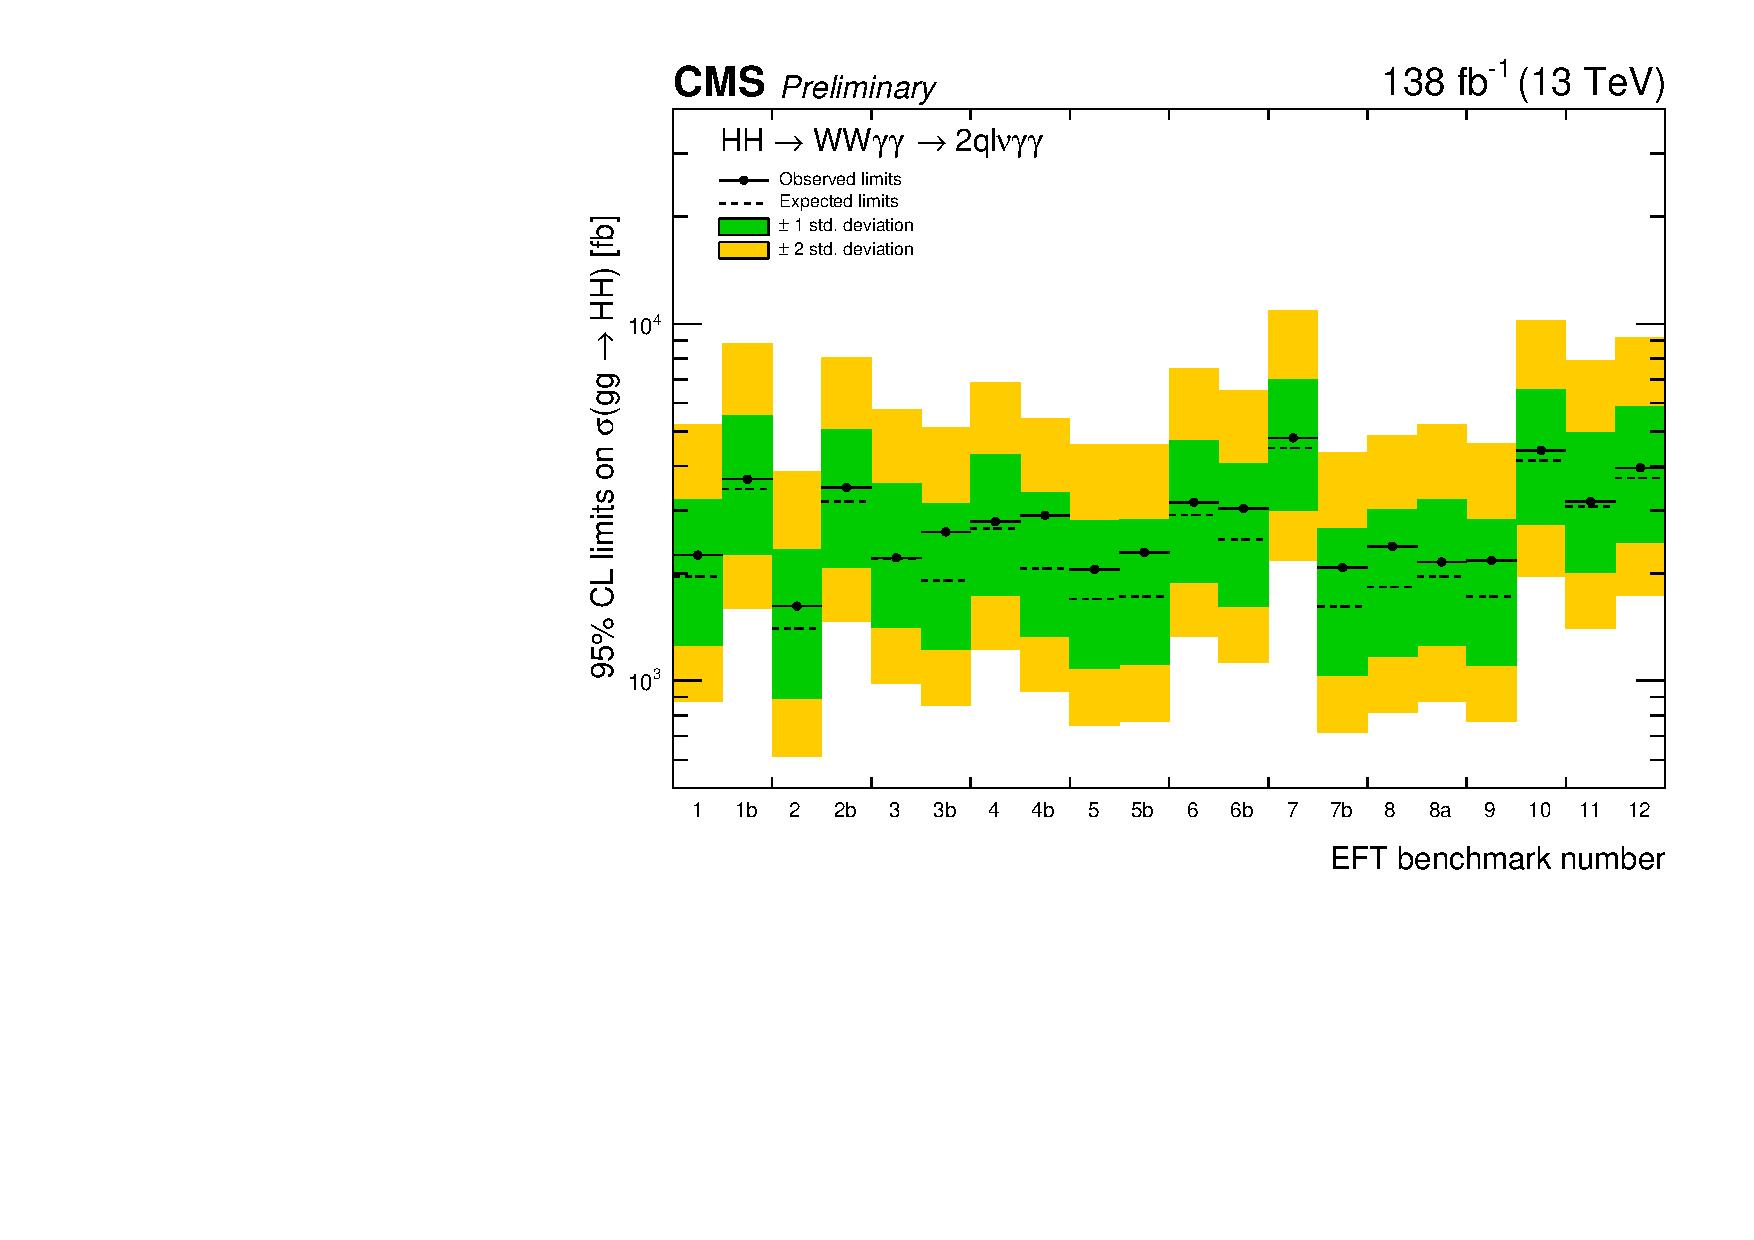
\includegraphics[width=0.45\textwidth]{Sections/HHWWgg/images/Results/EFT/EFT_SL_UpperLimit.pdf}}
    \qquad
    \subfloat[Fully-Leptonic channel]{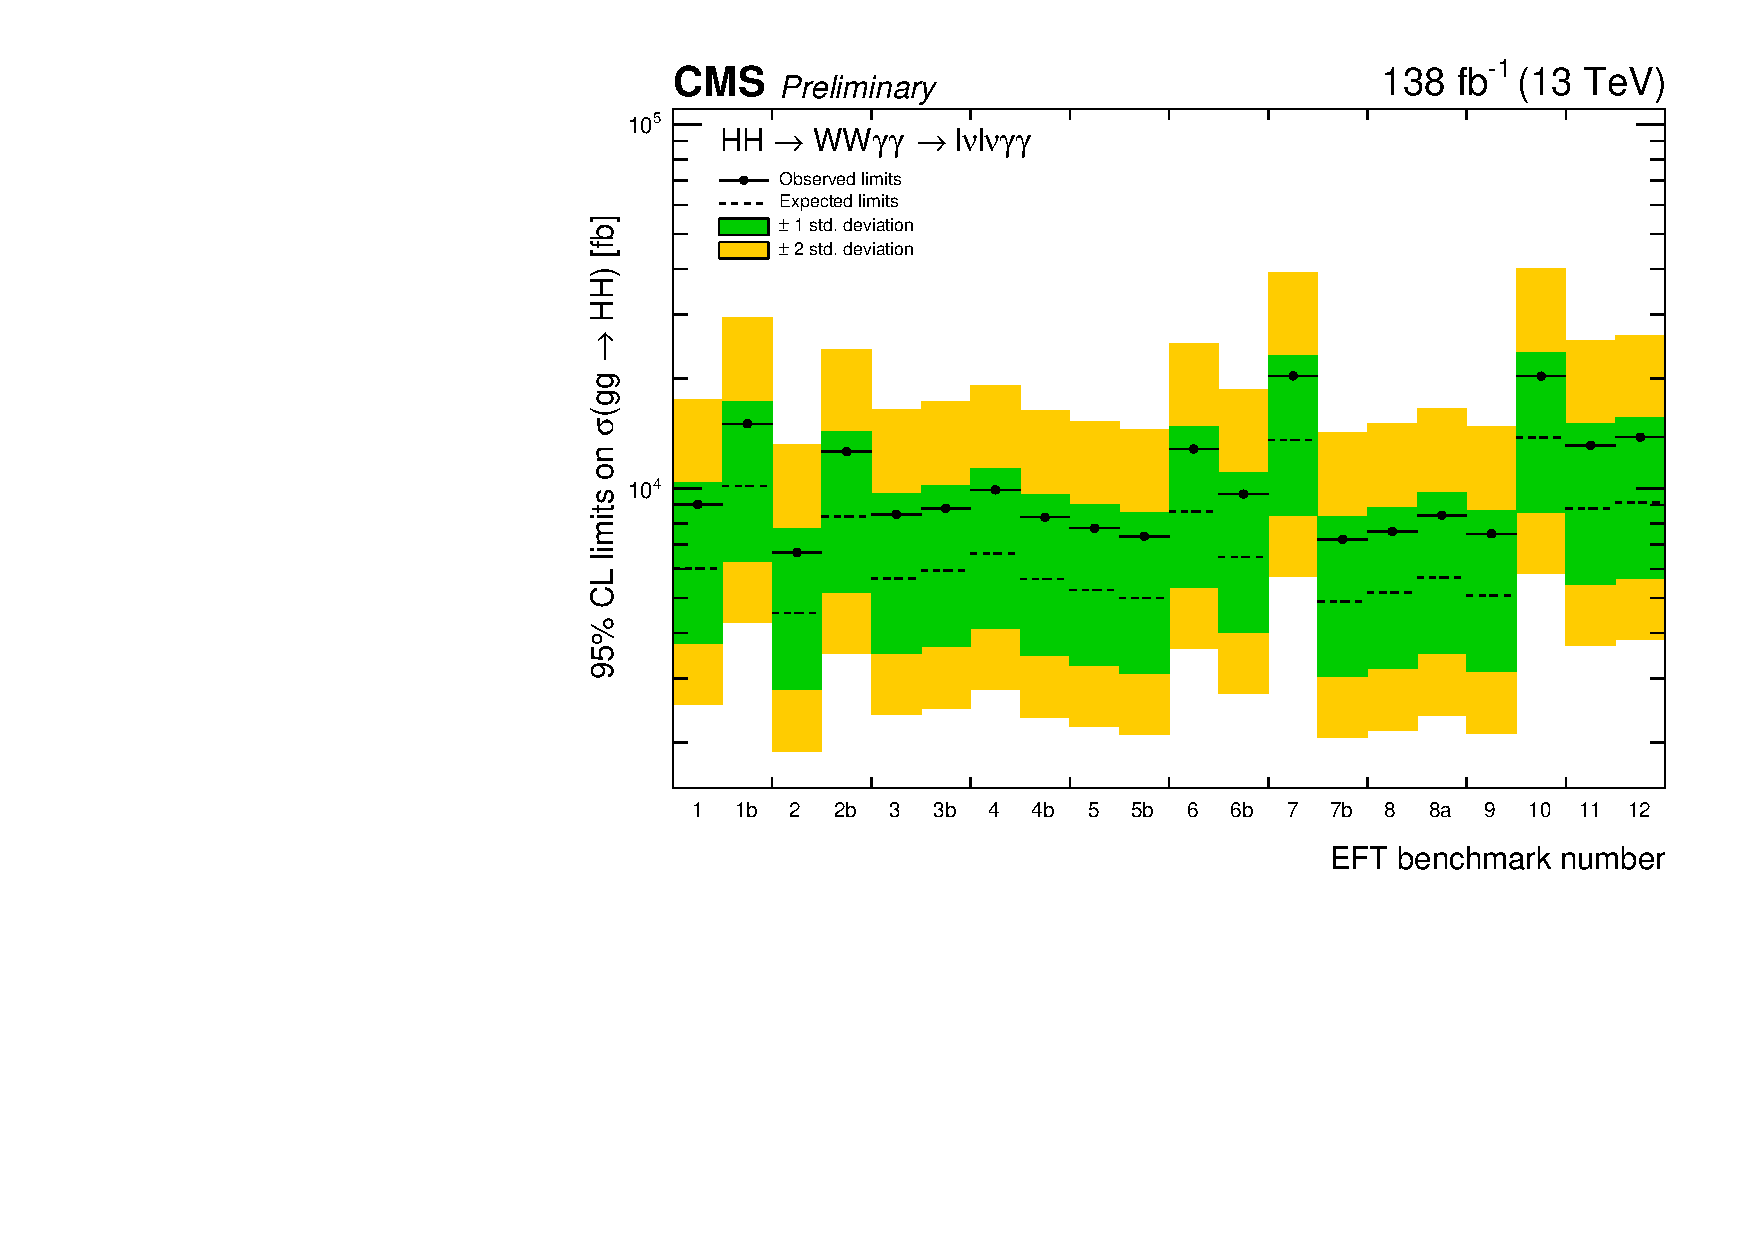
\includegraphics[width=0.45\textwidth]{Sections/HHWWgg/images/Results/EFT/EFT_FL_UpperLimit.pdf}}
    \qquad
    \subfloat[Fully-Hadronic channel]{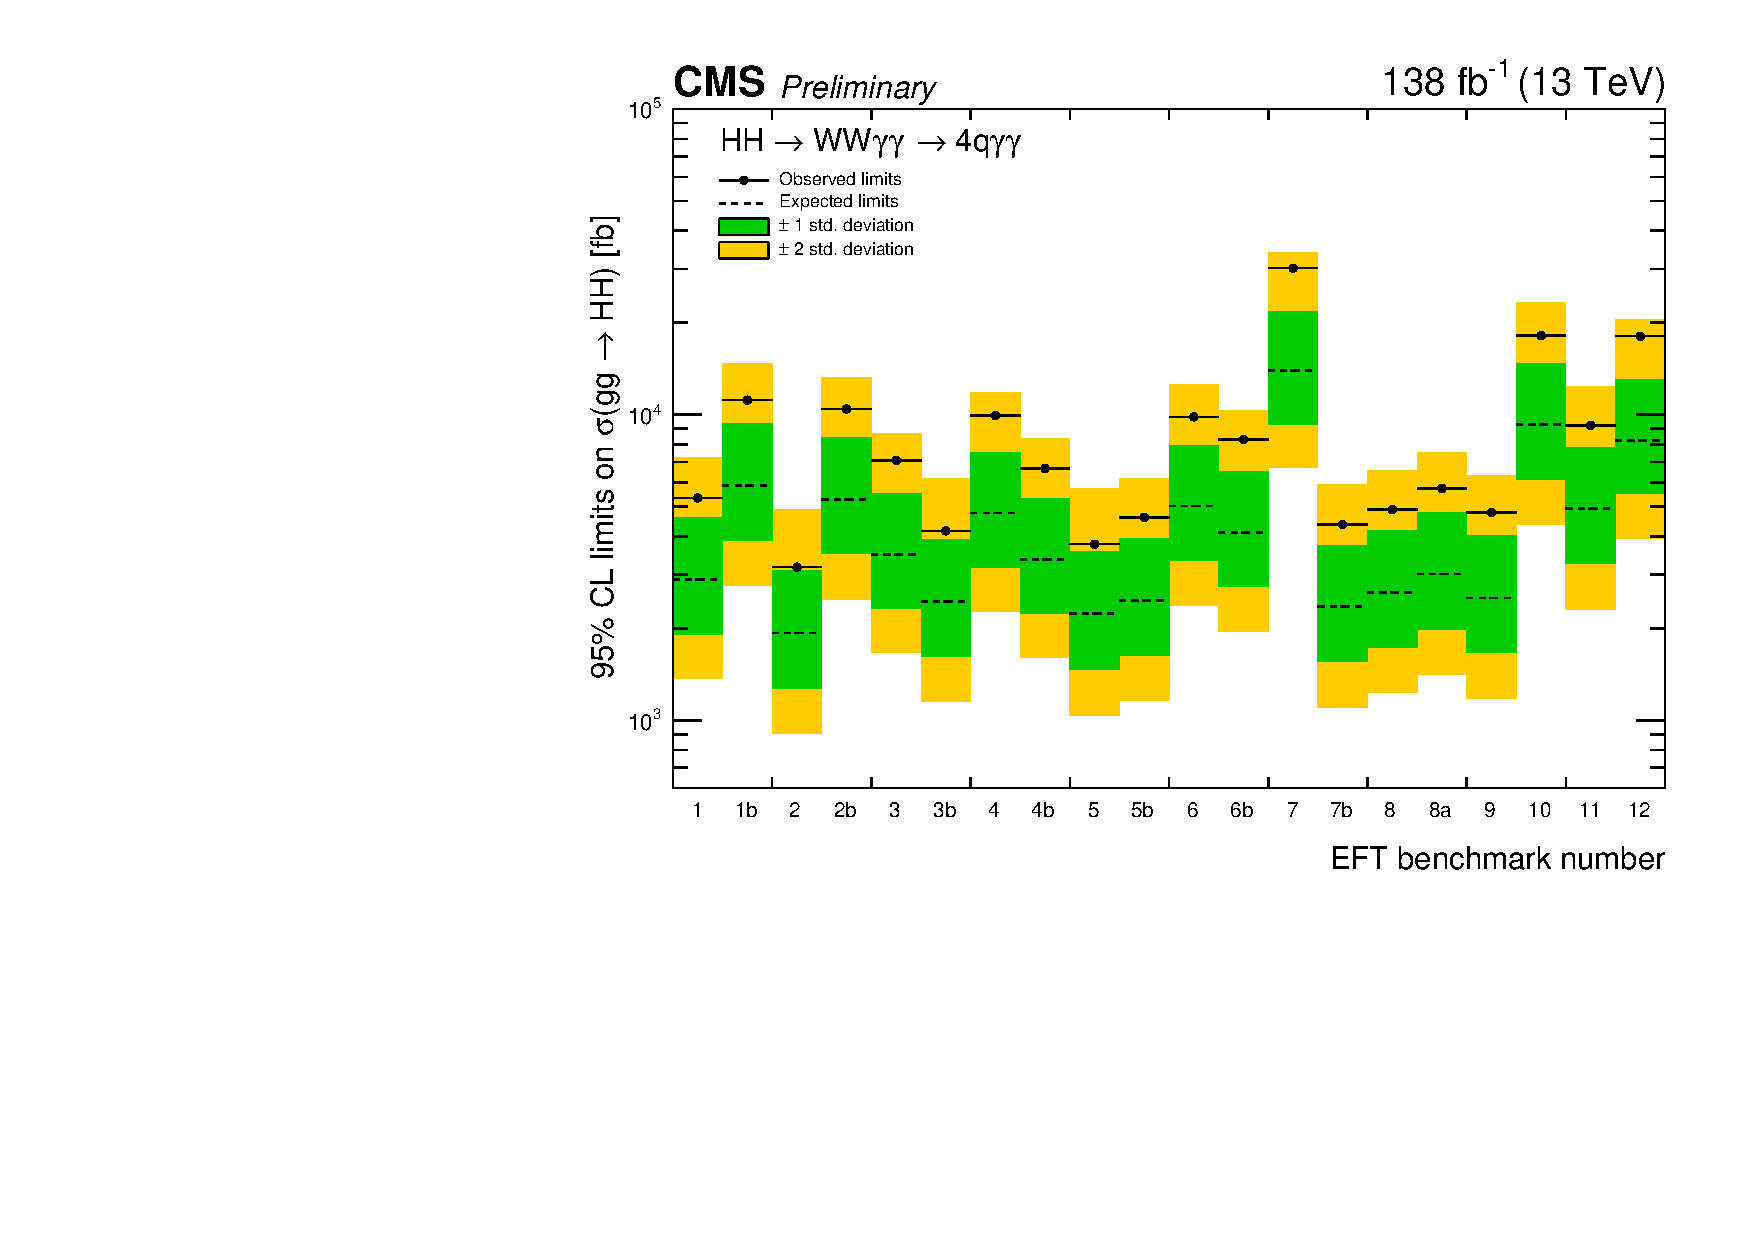
\includegraphics[width=0.45\textwidth]{Sections/HHWWgg/images/Results/EFT/EFT_FH_UpperLimit.pdf}}
    \caption{Run 2 95\% CL limits on HH gluon gluon fusion production for different nonresonant benchmark models defined in Table \ref{tab:eft_bench}.  }
    \label{fig:20_EFT_benchmark_results_perchannel}
\end{figure}


\begin{figure}[!htbp]
\centering
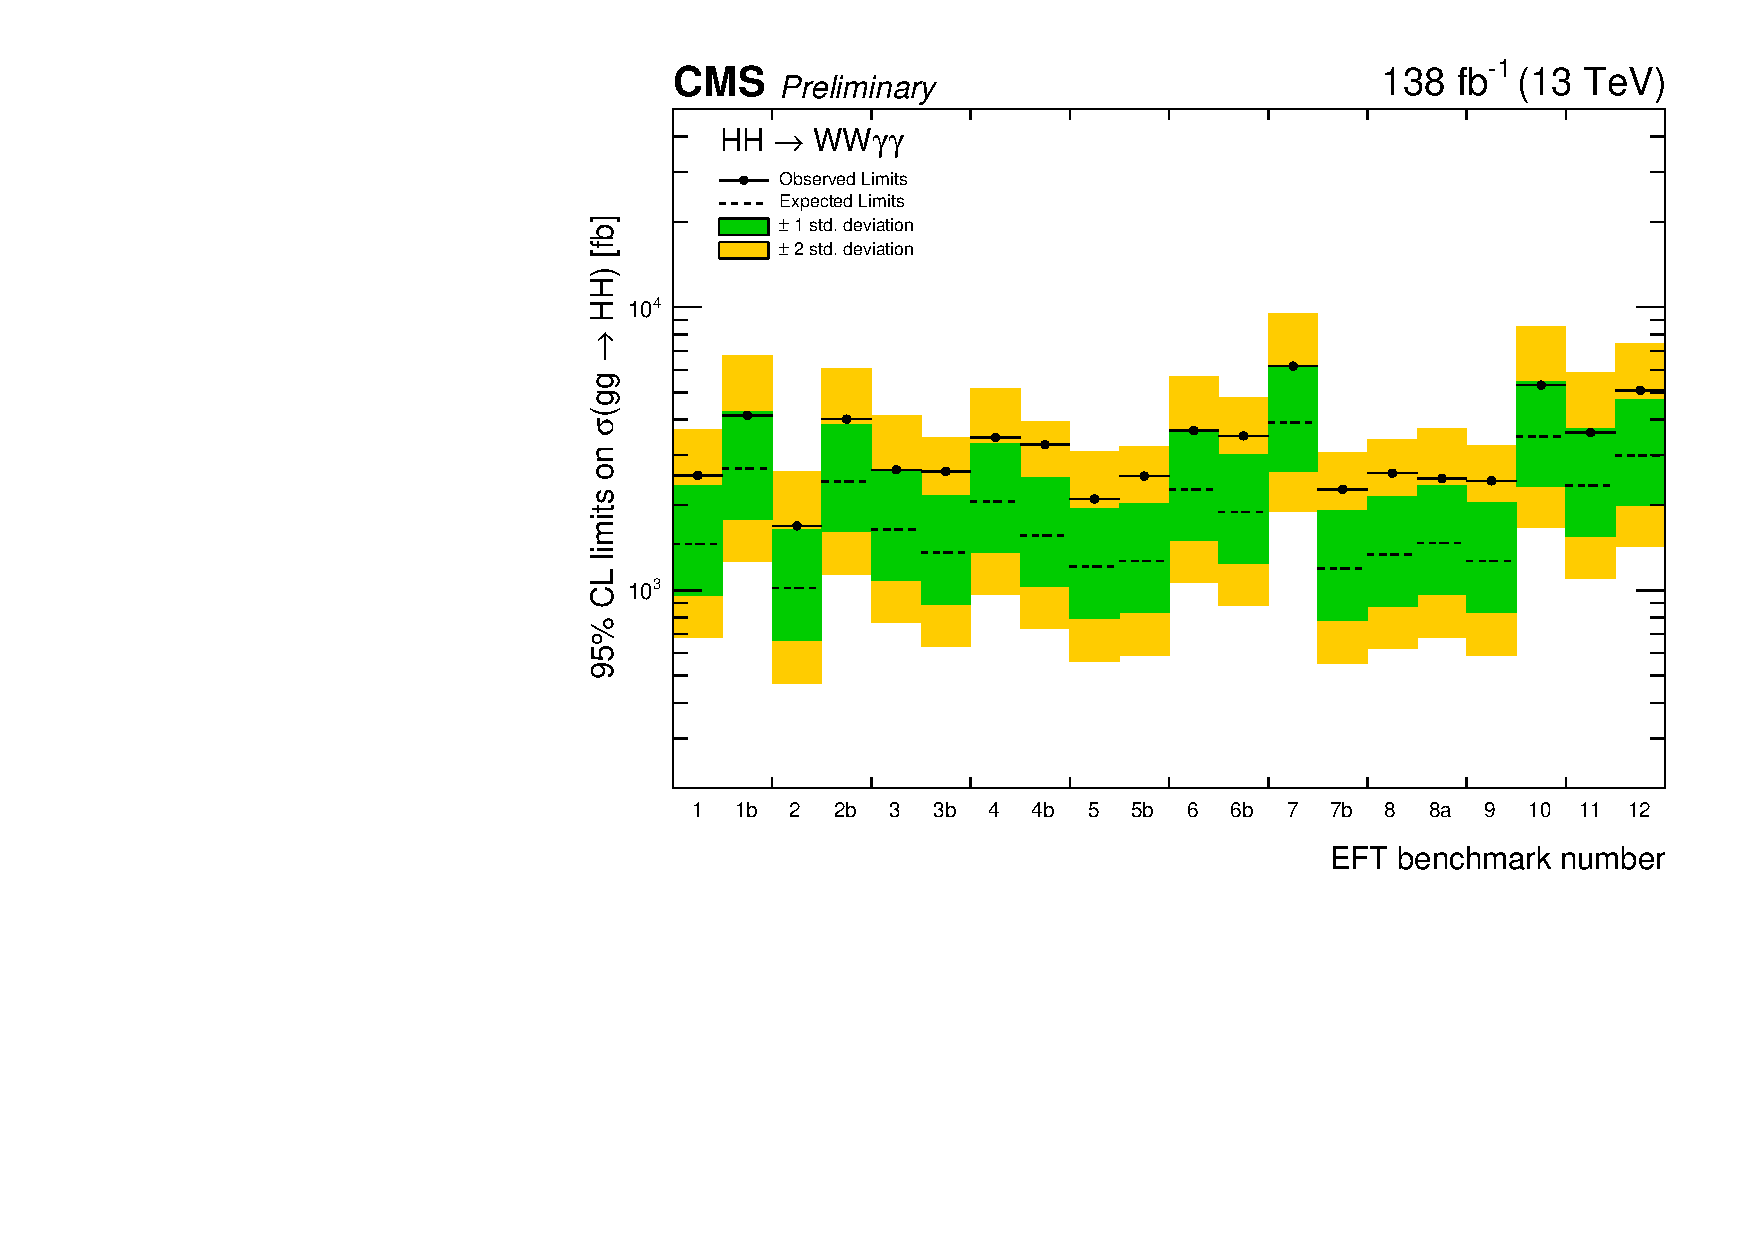
\includegraphics[width=0.75\textwidth]{Sections/HHWWgg/images/Results/EFT_CombinedUpperlimits.pdf}
\caption{Run 2 95\% $CL_{s}$ limits on HH gluon gluon fusion production for different nonresonant benchmark models defined in Table \ref{tab:eft_bench}.}
\label{fig:20_EFT_benchmark_results_all}
\end{figure}

